

\tikzset{every picture/.style={line width=0.75pt}} %set default line width to 0.75pt        

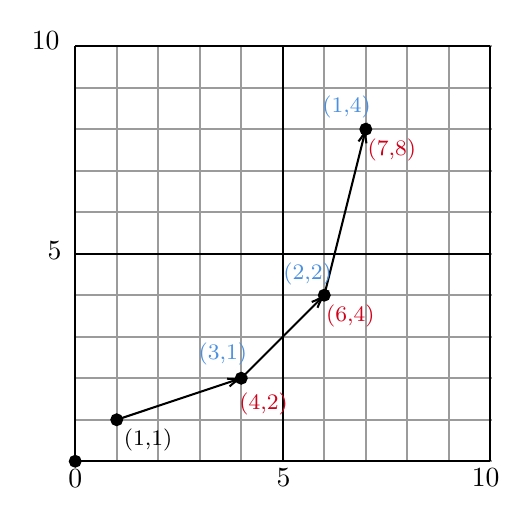
\begin{tikzpicture}[x=0.75pt,y=0.75pt,yscale=-1,xscale=1]
%uncomment if require: \path (0,300); %set diagram left start at 0, and has height of 300

%Shape: Grid [id:dp9135755721036088] 
\draw  [draw opacity=0] (100,66.2) -- (301,66.2) -- (301,266.5) -- (100,266.5) -- cycle ; \draw  [color={rgb, 255:red, 155; green, 155; blue, 155 }  ,draw opacity=1 ] (100,66.2) -- (100,266.5)(120,66.2) -- (120,266.5)(140,66.2) -- (140,266.5)(160,66.2) -- (160,266.5)(180,66.2) -- (180,266.5)(200,66.2) -- (200,266.5)(220,66.2) -- (220,266.5)(240,66.2) -- (240,266.5)(260,66.2) -- (260,266.5)(280,66.2) -- (280,266.5)(300,66.2) -- (300,266.5) ; \draw  [color={rgb, 255:red, 155; green, 155; blue, 155 }  ,draw opacity=1 ] (100,66.2) -- (301,66.2)(100,86.2) -- (301,86.2)(100,106.2) -- (301,106.2)(100,126.2) -- (301,126.2)(100,146.2) -- (301,146.2)(100,166.2) -- (301,166.2)(100,186.2) -- (301,186.2)(100,206.2) -- (301,206.2)(100,226.2) -- (301,226.2)(100,246.2) -- (301,246.2)(100,266.2) -- (301,266.2) ; \draw  [color={rgb, 255:red, 155; green, 155; blue, 155 }  ,draw opacity=1 ]  ;
%Straight Lines [id:da5428588612634048] 
\draw    (100,66.2) -- (100,266.2) ;
%Straight Lines [id:da8039381767256795] 
\draw    (100,66.2) -- (300,66.2) ;
%Straight Lines [id:da697248837047091] 
\draw    (300,266.2) -- (300,66.2) ;
%Straight Lines [id:da48495401334543176] 
\draw    (300,266.2) -- (100,266.2) ;
%Straight Lines [id:da712234155325812] 
\draw    (200,266.2) -- (200,66.2) ;
%Straight Lines [id:da13512977226752643] 
\draw    (100,166.2) -- (300,166.2) ;
%Shape: Circle [id:dp9308085386239336] 
\draw  [fill={rgb, 255:red, 0; green, 0; blue, 0 }  ,fill opacity=1 ] (97.4,266.2) .. controls (97.4,264.76) and (98.56,263.6) .. (100,263.6) .. controls (101.44,263.6) and (102.6,264.76) .. (102.6,266.2) .. controls (102.6,267.64) and (101.44,268.8) .. (100,268.8) .. controls (98.56,268.8) and (97.4,267.64) .. (97.4,266.2) -- cycle ;
%Shape: Circle [id:dp552388250536563] 
\draw  [fill={rgb, 255:red, 0; green, 0; blue, 0 }  ,fill opacity=1 ] (117.4,246.2) .. controls (117.4,244.76) and (118.56,243.6) .. (120,243.6) .. controls (121.44,243.6) and (122.6,244.76) .. (122.6,246.2) .. controls (122.6,247.64) and (121.44,248.8) .. (120,248.8) .. controls (118.56,248.8) and (117.4,247.64) .. (117.4,246.2) -- cycle ;
%Shape: Circle [id:dp8727246455385494] 
\draw  [fill={rgb, 255:red, 0; green, 0; blue, 0 }  ,fill opacity=1 ] (177.4,226.2) .. controls (177.4,224.76) and (178.56,223.6) .. (180,223.6) .. controls (181.44,223.6) and (182.6,224.76) .. (182.6,226.2) .. controls (182.6,227.64) and (181.44,228.8) .. (180,228.8) .. controls (178.56,228.8) and (177.4,227.64) .. (177.4,226.2) -- cycle ;
%Shape: Circle [id:dp2983524848929865] 
\draw  [fill={rgb, 255:red, 0; green, 0; blue, 0 }  ,fill opacity=1 ] (217.4,186.2) .. controls (217.4,184.76) and (218.56,183.6) .. (220,183.6) .. controls (221.44,183.6) and (222.6,184.76) .. (222.6,186.2) .. controls (222.6,187.64) and (221.44,188.8) .. (220,188.8) .. controls (218.56,188.8) and (217.4,187.64) .. (217.4,186.2) -- cycle ;
%Shape: Circle [id:dp25627201303944624] 
\draw  [fill={rgb, 255:red, 0; green, 0; blue, 0 }  ,fill opacity=1 ] (237.4,106.2) .. controls (237.4,104.76) and (238.56,103.6) .. (240,103.6) .. controls (241.44,103.6) and (242.6,104.76) .. (242.6,106.2) .. controls (242.6,107.64) and (241.44,108.8) .. (240,108.8) .. controls (238.56,108.8) and (237.4,107.64) .. (237.4,106.2) -- cycle ;
%Straight Lines [id:da34567719492876536] 
\draw    (120,246.2) -- (178.1,226.83) ;
\draw [shift={(180,226.2)}, rotate = 161.57] [color={rgb, 255:red, 0; green, 0; blue, 0 }  ][line width=0.75]    (6.56,-1.97) .. controls (4.17,-0.84) and (1.99,-0.18) .. (0,0) .. controls (1.99,0.18) and (4.17,0.84) .. (6.56,1.97)   ;
%Straight Lines [id:da106557243100044] 
\draw    (180,226.2) -- (218.59,187.61) ;
\draw [shift={(220,186.2)}, rotate = 135] [color={rgb, 255:red, 0; green, 0; blue, 0 }  ][line width=0.75]    (6.56,-1.97) .. controls (4.17,-0.84) and (1.99,-0.18) .. (0,0) .. controls (1.99,0.18) and (4.17,0.84) .. (6.56,1.97)   ;
%Straight Lines [id:da9122379405009994] 
\draw    (220,186.2) -- (239.51,108.14) ;
\draw [shift={(240,106.2)}, rotate = 104.04] [color={rgb, 255:red, 0; green, 0; blue, 0 }  ][line width=0.75]    (6.56,-1.97) .. controls (4.17,-0.84) and (1.99,-0.18) .. (0,0) .. controls (1.99,0.18) and (4.17,0.84) .. (6.56,1.97)   ;

% Text Node
\draw (95.2,268.8) node [anchor=north west][inner sep=0.75pt]   [align=left] {0};
% Text Node
\draw (195.6,268.2) node [anchor=north west][inner sep=0.75pt]   [align=left] {5};
% Text Node
\draw (289.6,268.2) node [anchor=north west][inner sep=0.75pt]   [align=left] {10};
% Text Node
\draw (85.2,159) node [anchor=north west][inner sep=0.75pt]   [align=left] {5};
% Text Node
\draw (77.6,57.8) node [anchor=north west][inner sep=0.75pt]   [align=left] {10};
% Text Node
\draw (122,249.2) node [anchor=north west][inner sep=0.75pt]  [font=\footnotesize] [align=left] {(1,1)};
% Text Node
\draw (177.6,231.8) node [anchor=north west][inner sep=0.75pt]  [font=\footnotesize,color={rgb, 255:red, 208; green, 2; blue, 27 }  ,opacity=1 ] [align=left] {(4,2)};
% Text Node
\draw (158,207.8) node [anchor=north west][inner sep=0.75pt]  [font=\footnotesize,color={rgb, 255:red, 74; green, 144; blue, 226 }  ,opacity=1 ] [align=left] {(3,1)};
% Text Node
\draw (219.4,189.2) node [anchor=north west][inner sep=0.75pt]  [font=\footnotesize,color={rgb, 255:red, 208; green, 2; blue, 27 }  ,opacity=1 ] [align=left] {(6,4)};
% Text Node
\draw (239.4,109.2) node [anchor=north west][inner sep=0.75pt]  [font=\footnotesize,color={rgb, 255:red, 208; green, 2; blue, 27 }  ,opacity=1 ] [align=left] {(7,8)};
% Text Node
\draw (198.8,169) node [anchor=north west][inner sep=0.75pt]  [font=\footnotesize,color={rgb, 255:red, 74; green, 144; blue, 226 }  ,opacity=1 ] [align=left] {(2,2)};
% Text Node
\draw (217.6,88.6) node [anchor=north west][inner sep=0.75pt]  [font=\footnotesize,color={rgb, 255:red, 74; green, 144; blue, 226 }  ,opacity=1 ] [align=left] {(1,4)};


\end{tikzpicture}
